\documentclass[main.tex,fontsize=8pt,paper=a4,paper=portrait,DIV=calc,]{scrartcl}
% Document
\usepackage[T1]{fontenc}
\usepackage[dvipsnames]{xcolor}
\usepackage[nswissgerman,english]{babel}
\renewcommand{\familydefault}{\sfdefault}

% Format
\usepackage[top=5mm,bottom=1mm,left=5mm,right=5mm]{geometry}
%\setlength{\headheight}{\baselineskip}
%\setlength{\headsep}{0mm}

%\usepackage{scrlayer-scrpage}
%\clearpairofpagestyles
%\chead{{\bfseries\TITLE, \AUTHOR, \pagename~\thepage}}

%\addtokomafont{pagehead}{\upshape}

\usepackage{multicol}
\setlength{\columnsep}{2mm}
\setlength{\columnseprule}{0.1pt}

% Math
\usepackage{amsmath}
\usepackage{amssymb}
\usepackage{amsfonts}

% Code
\usepackage{fancyvrb, etoolbox, listings, xcolor}
%\usemintedstyle{bw}

%\newminted[shell]{bash}{
%fontsize=\footnotesize,
%fontfamily=tt,
%breaklines=true,
%frame=single,
%framerule=0.1pt,
%framesep=2mm,
%tabsize=2
%}
%\newminted{css}{
%breaklines=true,
%tabsize=4,
%autogobble=true,
%escapeinside=||,
%stripall=true,
%stripnl=true,
%}

    \definecolor{lightgray}{rgb}{0.95, 0.95, 0.95}
    \definecolor{darkgray}{rgb}{0.4, 0.4, 0.4}
    \definecolor{purple}{rgb}{0.65, 0.12, 0.82}
    \definecolor{ocherCode}{rgb}{1, 0.5, 0} % #FF7F00 -> rgb(239, 169, 0)
    \definecolor{blueCode}{rgb}{0, 0, 0.93} % #0000EE -> rgb(0, 0, 238)
    \definecolor{greenCode}{rgb}{0, 0.6, 0} % #009900 -> rgb(0, 153, 0)
    \definecolor{teal}{rgb}{0.0, 0.5, 0.5}

\lstdefinestyle{code}{
    identifierstyle=\color{black},
    keywordstyle=\color{blue}\bfseries\small,
    ndkeywordstyle=\color{greenCode}\bfseries\small,
    stringstyle=\color{ocherCode}\ttfamily\small,
    commentstyle=\color{teal}\ttfamily\textit\small,
    basicstyle=\ttfamily\small,
    breakatwhitespace=false,         
    breaklines=true,                 
    captionpos=b,                    
    keepspaces=true,                 
    showspaces=false,                
    showstringspaces=false,
    showtabs=false,                  
    tabsize=2,
    belowskip=-5pt
}



% Images
\usepackage{graphicx}
\newcommand{\pic}{\includegraphics[scale=0.3]}
\graphicspath{{Screenshots/}{../Screenshots}}
\makeatletter
\def\pictext#1#2{%
    \@ifnextchar[{%
    \pictext@iiiii{#1}{#2}%
    }{%
      \pictext@iiiii{#1}{#2}[0.5,0.4,0.3]% Default is 5
    }%
}
\def\pictext@iiiii#1#2[#3,#4,#5]{\begin{minipage}{#3\textwidth}\includegraphics[scale=#4]{#1}\end{minipage}\begin{minipage}{#5\textwidth}#2\end{minipage}}
\def\minipg#1#2{%
    \@ifnextchar[{%
    \minipg@iiii{#1}{#2}%
    }{%
      \minipg@iiii{#1}{#2}[0.3,0.6]% Default is 5
    }%
}
\def\minipg@iiii#1#2[#3,#4]{\vspace{0.8mm}\begin{minipage}{#3\textwidth}#1\end{minipage}\begin{minipage}{#4\textwidth}#2\end{minipage}{\vspace{0.8mm}}}
\makeatother

%\newenvironment{minty}[2]% environment name
%{% begin code
%  \begin{minipage}{#1}
%  \begin{minted}{#2}
%}%
%{% end code
%  \end{minted}
%  \end{minipage}
%  \end{minty}\ignorespacesafterend
%} 

% Smaller Lists
\usepackage{enumitem}
\setlist[itemize,enumerate]{leftmargin=3mm, labelindent=0mm, labelwidth=1mm, labelsep=1mm, nosep}
\setlist[description]{leftmargin=0mm, nosep}
\setlength{\parindent}{0cm}

% Smaller Titles
\usepackage[explicit]{titlesec}

%% Color Boxes
\newcommand{\sectioncolor}[1]{\colorbox{black!60}{\parbox{0.989\linewidth}{\color{white}#1}}}
\newcommand{\subsectioncolor}[1]{\colorbox{black!50}{\parbox{0.989\linewidth}{\color{white}#1}}}
\newcommand{\subsubsectioncolor}[1]{\colorbox{black!40}{\parbox{0.989\linewidth}{\color{white}#1}}}
\newcommand{\paragraphcolor}[1]{\colorbox{black!30}{\parbox{0.989\linewidth}{\color{white}#1}}}
\newcommand{\subparagraphcolor}[1]{\colorbox{black!20}{\parbox{0.989\linewidth}{\color{white}#1}}}

%% Title Format
\titleformat{\section}{\vspace{0.5mm}\bfseries}{}{0mm}{\sectioncolor{\thesection~#1}}[{\vspace{0.5mm}}]
\titleformat{\subsection}{\vspace{0.5mm}\bfseries}{}{0mm}{\subsectioncolor{\thesubsection~#1}}[{\vspace{0.5mm}}]
\titleformat{\subsubsection}{\vspace{0.5mm}\bfseries}{}{0mm}{\subsubsectioncolor{\thesubsubsection~#1}}[{\vspace{0.5mm}}]
\titleformat{\paragraph}{\vspace{0.5mm}\bfseries}{}{0mm}{\paragraphcolor{\theparagraph~#1}}[{\vspace{0.5mm}}]
\titleformat{\subparagraph}{\vspace{0.5mm}\bfseries}{}{0mm}{\subparagraphcolor{\thesubparagraph~#1}}[{\vspace{0.5mm}}]

%% Title Spacing
\titlespacing{\section}{0mm}{0mm}{0mm}
\titlespacing{\subsection}{0mm}{0mm}{0mm}
\titlespacing{\subsubsection}{0mm}{0mm}{0mm}
\titlespacing{\paragraph}{0mm}{0mm}{0mm}
\titlespacing{\subparagraph}{0mm}{0mm}{0mm}

%% format cells
\usepackage[document]{ragged2e}
\usepackage{array, makecell}
\renewcommand{\arraystretch}{2}
\newcommand{\mc}{\makecell[{{m{1\linewidth}}}]}



\begin{document}
\begin{table}[h!]
\section{Unified Process}
\begin{tabular}{|m{0.975\linewidth}|}
\hline
\minipg{
The Unified Process is an iterative development strategy that focuses agility over structure.\newline
It does this by first broadly defining the scope of the project and creating Domain Models that only feature the most important usecases.
These usecases will then be implemented, tested and given to people for feedback.\newline
Based on this feedback the phase 2 Domain Model will be created with new features that will be implemented.\newline We still focus only the most important ones.\newline
We do this until the project reaches a releasable state. \\}
{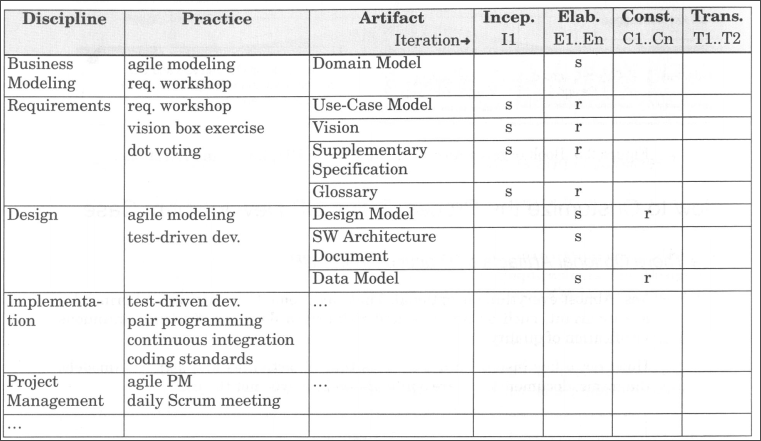
\includegraphics[scale=0.4]{2022-09-26-05:56:36.png}}[0.45,0.45]\\
\hline
\end{tabular}
\subsection{Phases of UP}
\begin{tabular}{|m{0,205\linewidth}|m{0.75\linewidth}|}
\hline
\textbf{\emph{Inception}} & Ceate a vision, scope, vague estimates and use cases.\\
\textbf{\emph{Elaboration}} & Create a refined vision, domain models, iterative implementation of core architecture, resolution of high risks, identification of most requirements and scope and more realistic estimates.\\
\textbf{\emph{Construction}} & Iterative implementation of remaining lower risk and easier elements, as well as preparation for deplyoment.\\
\textbf{\emph{Transition}} &beta tests and deplyoment \\
\hline
\end{tabular}
\section{Domain Models}
\subsection{Basic Terms}
\begin{tabular}{|m{0,205\linewidth}|m{0.75\linewidth}|}
\hline
\textbf{\emph{Requirement Analysis}} & Understand the general idea of the program, question is \textbf{What should it do?}\\
\hline
\textbf{\emph{Domain Analysis (OOA)}} & This is the first specification on how a program will accomplish something. It doesn't say anything about which functions to use etc, but what components are going to be used and how actors interact with each other. \newline For example, an online shop needs a shopping cart, some items to buy, an order list etc.\newline \textbf{This is done in UML} \newline \textbf{\color{red}{A Domain Model must be correct, complete and easy to understand \newline A Domain Model uses the conceptual model.}}\\
\hline
\textbf{Static View | Domain Model} & \minipg{The standard class UML diagram. \newline
Here we will have only the following three things:\newline \textbf{\color{red}{Attributes, classes and Associations}}}{\pic{2022-09-26:07:27:01.png}}[0.4,0.2]\\
\hline
\textbf{Dynamic View | Design Model} &  \minipg{Black-box Interaction Diagram or System Sequence Diagram for system operations.
\newline Contracts for system operations}{\pic{2022-09-26:07:39:58.png}}[0.4,0.2]\\
\hline
\end{tabular}
\subsection{Domain Model and Design Model}
\subsubsection{Domain Model}
\begin{tabular}{|m{0.975\linewidth}|}
\hline
\textbf{A Domain Model is the first representation of a vision. It should give the programmer a basic idea of how a program will be implemented, however it will not feature any specific code or functions.}\\
In general, this is about the problem, not the solution. \textbf{What, not how.}\\
\emph{A Domain Model is made of Conceptual Classes.}\\
\color{teal}{The idea is that \textbf{everyone involved in this project understands this model.}}\\
\hline
\end{tabular}
\end{table}
\begin{table}[h!]
\subsubsection{Design Model}
\begin{tabular}{|m{0.975\linewidth}|}
\hline
\textbf{This is derived from the Domain Model, it will be used to actually implement functions and specific interactions between the classes.}\\
\pic{2022-09-26:07:53:46.png}\\
\hline
\end{tabular}
\subsection{Steps for a Domain Model}
\begin{tabular}{|m{0.975\linewidth}|}
\hline
1. Read through the vision text quickly and note down \textbf{goals and key concepts}\\
2. Read the text carefully multiple times. Identify \textbf{classes, attributes and associations}\\
3. Improve the resulting domain model by \textbf{removing incorrect or redundant elements}\\
4. Read the text again to crosscheck your Model. Fix things if it isn't to the clients liking.\\
\hline
\end{tabular}
\subsection{Conceptual Classes}
\begin{tabular}{|m{0.975\linewidth}|}
\hline
-- \textbf{The naming of Conceptual Classes must be distinct}, there must not be confusion about what you mean with a class.\\
-- \textbf{Use Conceptual Classes if it is fundamental to the problem. If it is not, use an attribute.}\\
-- Conceptual classes should always be preferred over Attributes in case of doubt.\\
\hline
\textcolor{red}{The conceptual class consists of these 3 things}\newline
\begin{itemize}
\item \textbf{\emph{Symbol}} This is the box in UML alongside it's attributes.
\item \textbf{\emph{Intension}} This is the definition of said class, for example the definition of a window.
\item \textbf{\emph{Extension}} This is the real world usage of said class, door window, bathroom window, car window.
\end{itemize}\\
\hline
\end{tabular}
\subsection{Description Classes}
\begin{tabular}{|m{0.975\linewidth}|}
\hline
Often the actual Item is different from the description of said Item. For example, a Product has a description, however the item itself is independent of that description and can be used differently. For this reason we use description classes to explicitly state what is being affected.\\
\pic{2022-09-26:08:15:37.png}\\
\hline
\end{tabular}
\subsection{Transaction Classes}
\begin{tabular}{|m{0.975\linewidth}|}
\hline
Similar to Description Classes, transactions and interactions are also implemented better with proper dedicated classes.\newline
Think of a bank account, it makes no sense to conceptualize a transaction only with an association. \newline It would be much better to create a class for this transaction. \newline A major beneficial sideffect is the traceability of these transactions.\\
\pic{2022-09-26:08:18:34.png}\\
\hline
\end{tabular}
\end{table}
\pagebreak
\begin{table}[h!]
\subsection{Associations}
\begin{tabular}{|m{0.975\linewidth}|}
\hline
\minipg{
-- Associations are relationships between classes.\newline
-- Read association as follows: classname | association name | classname\newline
-- They always need a multiplicity, can have names, and can be used more than once for 2 classes.\newline
-- The baseline for Associations is that you should only specify what is necessary, avoid redundant information.\newline
-- Associations are always bidirectional, only the name can indicate a direction like: flies to ->.\newline
\color{teal}{if there is no direction specified, use default direction, top to bottom, left to right.} \newline
\textbf{Multiplicities: * zero or more, 1..* 1 or more, 1..40 one to 40, 5 exactly 5, 5,7,8 5 7 or 8}}
{\pic{2022-09-26:08:23:07.png}}[0.7,0.2]\\
\hline
\textbf{\textcolor{red}{Higher multiplicities should always be on top of lower multiplicities.}}\\
\hline
\minipg{\textbf{\textcolor{red}{Avoid * to * associations, often there is a missing class in the middle.}}}
{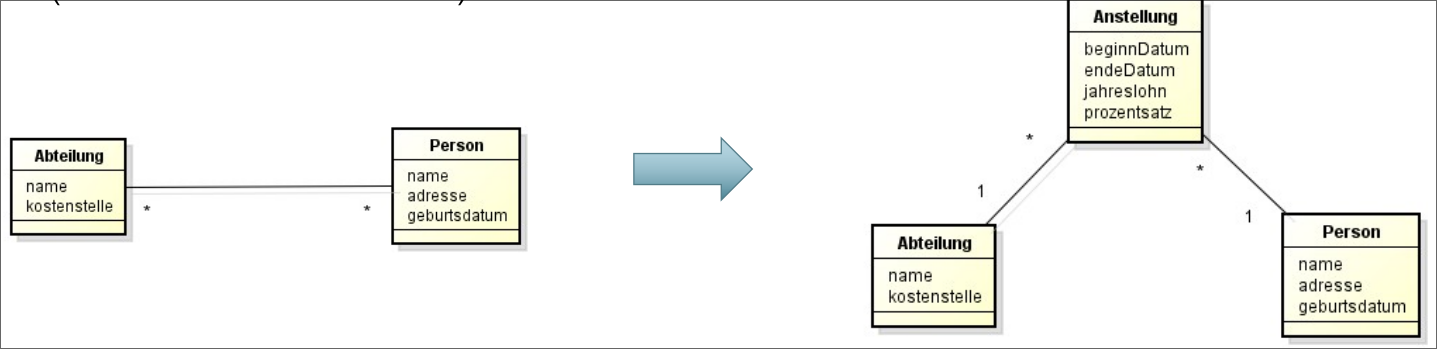
\includegraphics[scale=0.2]{2022-09-26-09:13:17.png}}[0.47,0.2]\\
\hline
\end{tabular}
\subsection{Attributes}
\begin{tabular}{|m{0.975\linewidth}|}
\hline
\minipg{
-- \textcolor{red}{Types are optional!} \newline
-- Attributes are simple datatypes \newline
-- Attributes are compared to each other by instance not by value. (even if values are the same!) \newline
}{\pic{2022-09-26-09:24:59.png}}[0.7,0.2]\\
\hline
\end{tabular}
\subsection{Generalization}
\begin{tabular}{|m{0.975\linewidth}|}
\hline
\minipg{
-- Generalization is simply the creation of superclasses. \newline
-- \textcolor{teal}{Superclasses can be abstract, in this case they are written in \emph{italics!}}\newline
}{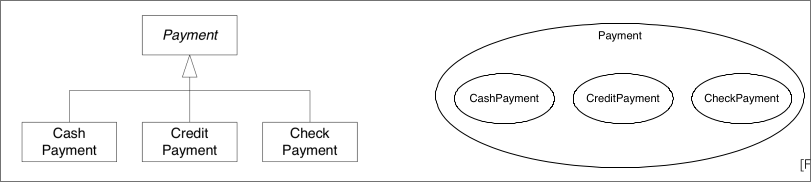
\includegraphics[scale=0.35]{2022-09-26-09:29:13.png}}[0.45,0.5]\\
\hline
\minipg{
-- \textcolor{teal}{Abstract superclasses can have attributes, \newline \,\,\,\,\,they will simply exist in the subclasses!}\newline
-- In this case subclasses will inherit all attributes from the superclass!
}{\pic{2022-09-26-09:29:23.png}}[0.5,0.4]\\
\hline
\end{tabular}
\section{States}
\begin{tabular}{|m{0.975\linewidth}|}
\hline
\minipg{
-- States should be implemented as it's own classes not as subclasses.\newline
-- If you have many states, using sublasses would make the model cluttered. \newline
-- It makes no sense either way, A transaction is not a different kind of transaction just because someone rejected it.
}{\pic{2022-09-26-09:38:53.png}}[0.6,0.3]\\
\hline
\end{tabular}
\begin{tabular}{|m{0,205\linewidth}|m{0.75\linewidth}|}
\hline
 & \\
\hline
\end{tabular}
\end{table}
\pagebreak
\begin{table}[h!]
\section{Requirements}
\subsection{Project Requirements vs Product Requirements}
\begin{tabular}{|m{0.977\linewidth}|}
\hline
The product deals with the actual requirements of our software, this means our app needs to be able to do x and y within z parameters.\newline
\textbf{This is usually referred to as "Work Product"}\newline
\textbf{\emph{In short Product requirement means Software Specification}}\newline
Project however deals with timelines, dates, costs, allocation, management, etc.\newline
\textbf{This is usually referred to as "Discipline"}\\
\hline
\end{tabular}
\subsection{Functional vs Non-Functional}
\begin{tabular}{|m{0.977\linewidth}|}
\hline
\vspace{2mm}
\begin{itemize}
  \item \textbf{\emph{Functional deals with \textcolor{red}{what} is needed}}
  \item \textbf{\emph{Non-Functional deals with \textcolor{red}{how well} it needs to work.}}
\vspace{-3mm}
\end{itemize}\\
\hline
\end{tabular}
\section{UseCases}
\subsection{Actors and Usecases}
\begin{tabular}{|m{0.205\linewidth}|m{0.75\linewidth}|}
\hline
\textbf{UseCases} & \minipg{
A usecase is a scenario that yields an \emph{observable result that is of value to an actor}.\newline
Each usecase is a \emph{sequence of actions} that a system executes.}
{\pic{2022-10-03-09:20:50.png}}[0.5,0.3]\\
\hline
\textbf{Actor} & \minipg{ 
Actors are not part of the System under Development (SuD)\newline
An actor plays a specific role of a user or another system that interacts with the SuD.\newline
A list of actors:\newline
\begin{itemize}
  \item Primary Actors (Users of the SuD)
  \item Supporting Actors (Third party system used in the SuD)
  \item Offstage Actors (Has an interest in the usecase but doesn't support it)
  \vspace{-3mm}
\end{itemize}}
{\pic{2022-10-03-09:20:57.png}
\vspace{10mm}
}[0.5,0.3]\\
\hline
\end{tabular}
\subsection{UseCase representations}
\begin{tabular}{|m{0.205\linewidth}|m{0.75\linewidth}|}
\hline
\textbf{\emph{Brief}} & 
This is the standard method of writing down a usecase. Here we only briefly write what is needed.\\
\hline
\textbf{\emph{Casual}} & 
Casual means that we find a middle ground between being elaborate and being brief...\newline
This is used for usecases that are more critical or harder to understand.\newline
It is normal to have more and more usecases in the casual style as development progresses.\newline
This is because everyone gets a clearer vision of what and how during development.\\
\hline
\textbf{\emph{Fully Dressed}} & 
This is only used for the most critical usecases and usescases that can't be understood otherwise.\\
\hline
\end{tabular}
\section{EBP Elementary Business Process}
\begin{tabular}{|m{0.977\linewidth}|}
\hline
\vspace{2mm}
\begin{itemize}
\item A task performed by one person in one place at one time, (single session)
\item response to a business event
\item adds measurable business value (Boss Test)
\item leaves the data in a consistent state
\vspace{-3mm}
\end{itemize}\\
\hline
\end{tabular}
\section{How to find UseCases}
\begin{tabular}{|m{0.977\linewidth}|}
\hline
\minipg{
\vspace{2mm}
\begin{enumerate}
  \item Fix the system boundary: Software, HW/SW-System, Entire Organisation?
  \item Identify primary actors and their goals: At the EBP level!
  \item Write down the use cases – first in the brief Format
\begin{itemize}
  \item Should satisfy primary actor goals
  \item 1 use case per primary actor goal
  \item Keep the UI out (essential style)
  \item Name the use case according to the goal, using a Verb + Object:
  \item \textbf{CRUD Create Read Update Delete} This can be represented as one usecase.
\end{itemize}
E.g. "ReturnCar", "CancelOrder"\newline
Recommendation: Use CamelCase to distinguish from natural language
\vspace{-3mm}
\end{enumerate}}
{\pic{2022-10-03-09:30:21.png}}[0.5,0.3]\\
\hline
\end{tabular}
\subsection{include and external}
\begin{tabular}{|m{0.205\linewidth}|m{0.75\linewidth}|}
\hline
\textbf{\emph{Include}} & \minipg{
These are sub-usecases when the usecase would otherwise be bloated.}
{\pic{2022-10-03-02:42:39.png}}[0.4,0.5]\\
\textbf{\emph{Extend}} & \minipg{
\,
}{\pic{2022-10-03-02:45:00.png}}[0.4,0.5]\\
\hline
\end{tabular}
\end{table}
\pagebreak
\begin{table}[ht!]
\subsection{User stories}
\begin{tabular}{|m{0.977\linewidth}|}
\hline
\textcolor{orange}{User stories do not have much in common with use cases, as it is specific to one user.\newline
They often are not representative of the experience of all users and need to be taken with a grain of salt.\newline Example: One user doesn't like gnome cuz no features, the other likes gnome cuz no bloat.}\\
\hline
\end{tabular}
\section{Non-Functional requirements continued}
\begin{tabular}{|m{0.2\linewidth}|m{0.755\linewidth}|}
\hline
Types of non-functional requirements &
\textcolor{orange}{The bare minimum of non-functional requirements are the following:}\newline
\begin{itemize}
  \item \textcolor{teal}{Performance:} max response times, fps etc 
  \item \textcolor{teal}{Scalability:} max amount of users, max data volume etc
  \item \textcolor{teal}{Constraints:} programming language used, database
  \vspace{-3mm}
\end{itemize}\\
\hline 
Verification & 
\textcolor{orange}{Non-functional requirements should always be verifiable, this is usually done with \textbf{testing} and \textbf{reviewing}.}\\
\hline
Relevance & 
\textcolor{orange}{Non-Functional requirements should always be relevant to your task. Don't create tests for features you won't really need.}\\
\hline
\end{tabular}
\subsection{FURPS}
\begin{tabular}{|m{0.977\linewidth}|}
\hline
\textcolor{orange}{FURPS is simply a collection of other requirements that can also be used if they are relevant}\newline
\begin{itemize}
  \item \textcolor{teal}{Functionality} error handling, logging, authentication etc
  \item \textcolor{teal}{Usability} accessibility -> colors, visuals etc
  \item \textcolor{teal}{Reliability} ex: a non crashing video editor
  \item \textcolor{teal}{Performance} task xy takes less than z seconds
  \item \textcolor{teal}{Supportability} ease of support
  \item \textcolor{teal}{Others} Hardware and software constraints, licensing
  \vspace{-3mm}
\end{itemize} \\ 
\hline
\end{tabular}
\end{table}
\pagebreak
\begin{table}[ht!]
\section{Graphs}
\begin{tabular}{|m{0.977\linewidth}|}
\hline
\minipg{
A graph is a datastructure with \textbf{edges} and \textbf{Nodes}.\newline
There can be different versions of graphs:\newline
\begin{itemize}
  \item \emph{undirected}, this means the edges have no direction from and to each other
  \item \emph{directed}, this means the edges have a direction from and to each other
  \item \emph{Acyclic}, No node is reachable from itself
\end{itemize}
Graphs specially handle \textbf{Dependencies and Causality} well \newline
Trees and lists are \emph{special cases of Directed Acyclic Graphs, DAG}.}
{\pic{2022-10-10:07:45:45.png}}[0.5,0.4]\\
\hline
\end{tabular}
\section{Version Control / Git}
\begin{tabular}{|m{0.2\linewidth}|m{0.755\linewidth}|}
\hline
Version Control Systems & \minipg{
Git uses distributed style, \newline 
since you can create branches on your own pc locally,\newline
but then also push this to a server!
}
{\pic{2022-10-10:08:02:03.png}}[0.25,0.5]\\
\hline
Git standard facts &
developed by torvalds in 2005.\newline
Uses "snapshots" -> commits to handle version control.\newline
\textcolor{teal}{Git is represented by a \textbf{DAG}, \textbf{Nodes are commits and edges are the parent reference.}}\newline
\textbf{SHA-1 hashes} used for indexing and integrity\\
\hline
\textbf{Snapshot vs Delta} &
\textcolor{teal}{Snapshots store the entire projects as a hash in each iteration.}\newline
\textcolor{orange}{Delta based systems only store the changes of each iteration.}\newline
Theoretically delta systems are faster in terms of merging, but it makes collaboration harder! -> forking\\
\hline
Commits & 
\textbf{0 parents -> root}, \textbf{1 parent -> regular commit}, or \textbf{multiple parents -> merge commit from fork}.\\
\hline
Git File Status & \minipg{
There are different states that a file can be in:
\begin{itemize}
\item \textcolor{red}{Modified} \textcolor{teal}{simply save a change locally}
  \item \textcolor{yellow}{Staged} Modifications planned for next commit \textcolor{teal}{git add -A}
  \item \textcolor{green}{Committed} Modifications stored \textcolor{teal}{git commit -m "ping pang"}
\end{itemize}
\, \newline
There are different sections in a git project:
\begin{itemize}
  \item Working Directory
  \item \textcolor{yellow}{Staging area} aka. index
  \item \textcolor{green}{Repository} aka. Git directory
\end{itemize}
\, \newline}{\pic{2022-10-10:08:16:11.png}}[0.4,0.5]\\
\hline
  \textbf{Semantic Commit Messages} & \textcolor{teal}{ 
feat: add hat wobble\newline
\char`\^ --\char`\^  \, \char`\^ -----------------\char`\^ \newline
|     | \newline
|     + -> Summary in present tense.\newline
|\newline
+ ------> Type: chore, docs, feat, fix, refactor, style, or test.}\newline
\, \newline
These are a few of the possible messages:\newline
\begin{itemize}
  \item feat: (new feature for the user, not a new feature for build script)
  \item fix: (bug fix for the user, not a fix to a build script)
  \item docs: (changes to the documentation)
  \item style: (formatting, missing semi colons, etc; no production code change)
  \item refactor: (refactoring production code, eg. renaming a variable)
  \item test: (adding missing tests, refactoring tests; no production code change)
  \item chore: (updating grunt tasks etc; no production code change)
\end{itemize}\\
\hline
\textbf{commands} &
\vspace{2mm}
\begin{itemize}
\item \textcolor{teal}{git add init} \indent initialize repository
\item \textcolor{teal}{git clone url} \indent clone a remote repos
\item \textcolor{teal}{git status} \indent check if any changes are made locally or remote
\item \textcolor{teal}{git log} \indent show commit log
\item \textcolor{teal}{git remote add origin url} \indent add remote repos from github/gitlab
\item \textcolor{teal}{git remote add upstream url} \indent add upstream repos to merge from
\item \textcolor{teal}{git remote remove origin/upstream} \indent remove a remote repos
\item \textcolor{teal}{git add -A/file} \indent stage a file
\item \textcolor{teal}{git remove -A/file} \indent unstage a file
\item \textcolor{teal}{git commit -S -m "message"} \indent sign and commit changes
\item \textcolor{teal}{git stash} \indent stash current changes
\item \textcolor{teal}{git stash clear} \indent clear stash
\item \textcolor{teal}{git push remotename branchname} \indent push to remote repos
\item \textcolor{teal}{git pull remotename branchname} \indent pull from remote repos
\item \textcolor{teal}{git fetch remotename branchname} \indent download hashes for changes, !!but not the files!!
\item \textcolor{teal}{git difftool} \indent show gitdiff from staged to current commit
\item \textcolor{teal}{git mergetool} \indent tool to merge 2 commits that have conflicts
\item \textcolor{teal}{git checkout branch/commit} \indent go to a certain branch or commit
\item \textcolor{teal}{git switch branch/commit} \indent go to a certain branch \textcolor{red}{!! with changes from current branch !!}
\item \textcolor{teal}{git tag v1.0} \indent human friendly alias for commit (makes it easier to navigate to this commit)
\item \textcolor{teal}{git rebase branchname} \indent essentially a merge with the target branch on your side, often used to update pull requests
\item \textcolor{teal}{git reset --soft HEAD\char`\~ amount of commits} \indent removes a commit from the branch without changing the files \newline
\textcolor{red}{!! remote changes will however be removed !!}\newline
\item \textcolor{teal}{git reset --hard HEAD\char`\~ amount of commits} \indent removes a commit from the branch \textcolor{red}{!! and removes the files !!}
\vspace{-3mm}
\end{itemize}\\
\hline
\end{tabular}
\end{table}
\pagebreak
\begin{table}[ht!]
\begin{tabular}{|m{0.2\linewidth}|m{0.755\linewidth}|}
\hline
Definition of Branch & 
\textcolor{orange}{A branch is an \textbf{active line of development}.}\newline
In human speak: It is a space to develop something, and then later merge it to another branch, aka git......\\
\hline
Two way merges & 
\textcolor{orange}{With two way merges we do not know what we want to keep, as 2 users have made changes to a single line, this can't be merged automatically. \newline
The reason for this is that with a two way merge, we do not have a common ancestor, therefore we can't know which one the update was, simply using dates is not the answer!}\\
\hline
Three way merge & 
\textcolor{orange}{Three way merges are what we do in reality, it has a base branch and 2 newer branches that will update the base branch.\newline
Here we can update automatically as long as the 2 new branches will not work on the same line!}\newline
\pic{2022-10-24:07:52:34.png}\\
\hline
Development Branches vs Feature Branches & 
\textcolor{orange}{The difference between dev branches and feature branches are simply the fact that features branches usually do not get merged, instead they will stand as their independent branch for people who want to use this said feature. \newline
Usually this is only used for stable vs unstable branches, as well as version branches and topics.}\\
\hline
Rebase &
\textcolor{orange}{The result in terms of files is the same as merging, \textbf{but, the ancestor changes! Hence the name rebase},\newline
This is used to update your branch when you work on a feature, or if you need to change the branch that you are basing your current branch on.\newline
Eg. you work on voice activation and notice that you need to change the ancestor from main to group-call :)}\newline
\textcolor{red}{This is more clean in comparison to merging when updating a branch!}\newline
\textcolor{teal}{Don't rebase to other repositories, should be common sense, but you never know.}\\
\hline
Distributed Version Control &
\textcolor{orange}{The only real change is in the "server", before we talked about local repositories and the server repository. \newline
Now we can have a variable amount of "servers", making it distributed. \newline
Each instance is still a \textbf{DAG of commits}.}\newline
\, \newline
\textcolor{purple}{The way we talk about the instances is \textbf{remotes}, hence the command git remote.\newline
You have various ways of setting these up like https, ssh and more. Here ssh is the most flexible one.}\\
\hline
Centralized Workflow & 
\textcolor{orange}{Here the developers all have access to one singular repository. Usually this is used for internal projects that aren't open to the rest of the world.\newline
This workflow is not distributed, as the developers only have their changes on their working pc and commit locally.}\\
\hline
Integration-Manager Workflow & 
\textcolor{orange}{Here each developer has a fork of the main repository, then the developers create pull requests of the main repository.\newline
This gives you more control over what changes get upstreamed, it can work with open source worklow, and the developers can work on their changes on multiple pcs, as they essentially have their own version of the project.}\\
\hline
\end{tabular}
\end{table}
\pagebreak
\begin{table}[ht!]
\section{State Machine Diagrams}
\begin{tabular}{|m{0.2\linewidth}|m{0.755\linewidth}|}
\hline
Generic Definition & 
\textcolor{orange}{The base idea is a machine that has different behaviors dependent on the current state, that the machine is in at a given time.}\newline
\textcolor{red}{Important Notes:}\newline
\textcolor{purple}{\indent With state machines, every object needs to have a state at every point, there can't be objects that have no state, otherwise it would obviously not be a state machine anymore. \newline
\indent With uml state machines, you don't always need a final state like with DFAs and NFAs, this is usually because modern system often go into a standby rather than being done for good.}\newline
\textcolor{teal}{State Machines are useful in a variety of cases:}\newline
\begin{itemize}
\item \textcolor{teal}{Domain analysis}
\item \textcolor{teal}{Requirements analysis}
\item \textcolor{teal}{Design}
\item \textcolor{teal}{Sometimes even implementation}
\vspace{-3mm}
\end{itemize}\\
\hline
Scope & 
\textcolor{orange}{\textbf{The scope can be anything with a state dependent behavior.}}\newline
This could be something like a light switch, a bug report, etc.\\
\hline
Notation & 
\textcolor{orange}{There are different notations to state machines, for example DFAs and NFAs from Automata\newline
However for this module, we will use UML notation}\newline
\minipg{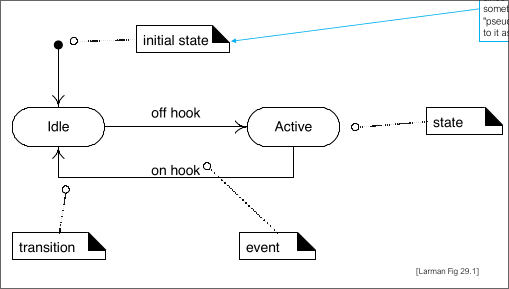
\includegraphics[scale=0.4]{2022-10-31-08:31:35.png}\newline
}{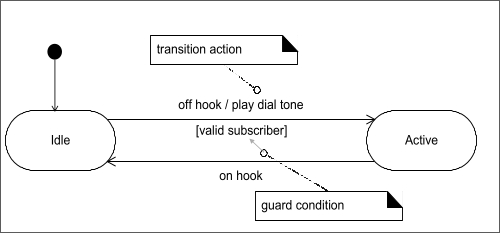
\includegraphics[scale=0.4]{2022-10-31-08:40:28.png}}[0.4,0.4]\\
\hline
Transition &
\vspace{2mm}
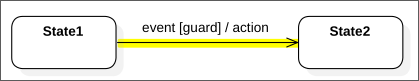
\includegraphics[scale=0.4]{2022-10-31-08:52:11.png}\newline
\textcolor{red}{Legend:}\newline
\begin{itemize}
\item \textcolor{teal}{event: The event that has triggered the transition}
\item \textcolor{teal}{[guard]: an if statement on the event}
\item \textcolor{teal}{action: an action that can be performed on the transition}
\vspace{-3mm}
\end{itemize}\\
\hline
Events & 
\textcolor{orange}{Events are always \textbf{instant and sequential}, they occur \textbf{outside of the system in consideration.}\newline
They can be viewed as a message or signal that the system receives.}\newline
\textcolor{purple}{\textbf{No event trigger means that the transition is ALWAYS triggered!}}\\
\hline
Guards & 
\textcolor{orange}{The enabling boolean expression for the event.\newline
Typically refers to: \newline
Extended state variables or some internal or external state.}
\\
\hline
Actions & 
\textcolor{orange}{Actions are \textbf{atomic and can't be interrupted}.\newline
Typically an \textbf{imperative command}, that involves sending a message or updating an extended state variable.}\newline
\textcolor{purple}{We define entry \textbf{entry actions} and \textbf{exit actions} in order for us to have more flexibility when writing and reading the state diagram.\newline
Actions can be composed/chained with a \textbf{\textit{;}} -> count := count + 1; something else;}\\
\hline
Nested State Machines & 
\textcolor{orange}{You can always create a state machine inside another state machine in order to have even more modularity.\newline
For example you might have an on-off state, then inside the on state you have an entire new system that does something else when on and things happen.}\newline
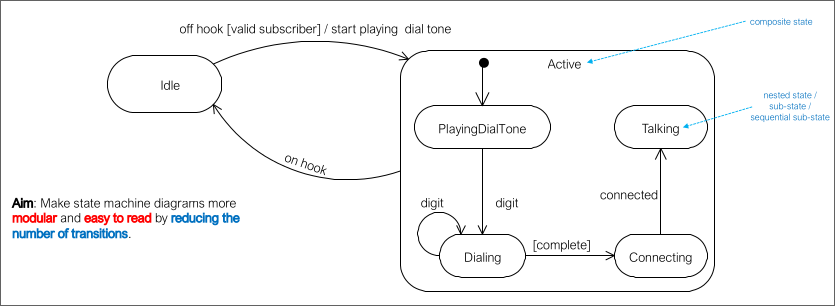
\includegraphics[scale=0.45]{2022-10-31-09:24:04.png}\newline
\textcolor{purple}{Here you can see the phone statemachine and another one inside it.\newline
Should you be inside the right statemachine, you can always exit from this and go back to the outside state machine, aka from connecting to idle by pressing cancel or something similar.}\\
\hline
\end{tabular}
\end{table}
\pagebreak
\begin{table}[ht!]
\begin{tabular}{|m{0.2\linewidth}|m{0.755\linewidth}|}
\hline
Creation of a State Machine & 
\vspace{2mm}
\begin{enumerate}
  \item \textcolor{purple}{Read through the description quickly,\newline
    Decide on the \textbf{object} and the \textbf{level of abstraction}}
  \item \textcolor{purple}{Read through the description \textbf{carefully, multiple times and:}}\newline
    \begin{itemize}
    \item \textcolor{teal}{Identify the relevant \textbf{states}}
    \item \textcolor{teal}{Identify all possible \textbf{events}}
    \item \textcolor{teal}{Identify and draw in \textbf{all relevant transitions}}
    \item \textcolor{teal}{Identify and draw in \textbf{all guards}}
    \item \textcolor{teal}{Identify and draw in \textbf{all actions}}
    \item \textcolor{teal}{Simplify the diagram using \textbf{nested states}}
    \item \textcolor{teal}{Simplify the diagram using \textbf{extended state variables}}
    \vspace{-3mm}
    \end{itemize}
\end{enumerate}\\
\hline
\end{tabular}
\section{Software Testing}
\begin{tabular}{|m{0.2\linewidth}|m{0.755\linewidth}|}
\hline
Basics & 
Software testing is part of the \textbf{dynamic techniques}, meaning it is used on the running software.\newline
Software testing is done to \textbf{show defects of software, not the absence of it!}.\newline
In contrast to trial and error, it is \textbf{done with clear intention and systematically, reproducable and traceable!}\newline
Requirements for software testings:\newline
\begin{itemize}
\item \textcolor{purple}{Planned} \newline
  Who does what, when and how?
\item \textcolor{purple}{Systematically specified}\newline
  \textbf{Test Specification}
\item \textcolor{purple}{Results documented} \newline
  \textbf{Test Protocol}
\vspace{-3mm}
\end{itemize} \\
\hline
Problem with Software Testing & 
Usually we build software with some sort of input, this makes the possbility of results infinite! \newline
How do we create a program that will work with the infinite inputs that we could get?
\begin{itemize}
\item \textcolor{purple}{Grouping inputs}\newline
  Many inputs are very similar, for example, if the program works for 5 numbers,\newline
  chances are that the input works for yet another number
\item \textcolor{purple}{Modularization}\newline
  This means \textbf{testing classes directly, testing packages directly and testing the system directly}
\vspace{-3mm}
\end{itemize}\\ 
\hline
Different types of "failures" &
\vspace{2mm}
\begin{itemize}
\item \textcolor{orange}{Error}\newline
  A human action that produces an incorrect result
\item \textcolor{orange}{Defect}\newline
  A flaw in a compnent or system that can cause it fo fail to perform its required function.
\item \textcolor{orange}{Failure}\newline
  Deviation of the component or system from its expected behavior.
\item \textcolor{orange}{defect}\newline
  if encountered during exectuion, may casue a \textbf{failure} of the component or the system
\item \textcolor{teal}{False-positive result}\newline
  A test that shows either a good result or a bad result, but it might be skewed due to other issues.
\vspace{-3mm}
\end{itemize} \\
\hline
Test Specification & 
This simply says what the \textbf{precondition} is, what the \textbf{input} is, and what the \textbf{expected output} is.\newline
\textcolor{red}{These are typically \textbf{used for system tests}, which are often done \textbf{manually!!}}\newline
\begin{tabular}{|l|l|l|l|l|}
\hline
Nr. & Description of Test Case & Precondition & Input/Interaction & Expected Output \\
\hline
1 & test sum & User selected\newline sum function & 5, 7, 3, 7 & 22 \\
\hline
\end{tabular}
\vspace{2mm}\\
\hline
Test Protocol & 
This simply documents the test procedure.\newline
\begin{tabular}{|l|l|l|l|l|}
\hline
Nr. & Description of Test Case & Precondition & Input/Interaction & Expected Output \\ 
\hline
1 & test sum & User selected sum function & 5, 7, 3, 7 & 22 \\
\hline
\end{tabular}
\vspace{2mm}
\begin{tabular}{|l|l|l|}
\hline
Actual Output & Test passed / failed & Tester, Time, Date\\ 
\hline
20 & failed & Dashie, 2pm, 11.11.2022\\
\hline
\end{tabular}
\vspace{2mm} \\
\hline
Types of Testing & 
We differentiate \textbf{functional testing}, \textbf{perfromance testing} and \textbf{usability testing}.\\
\hline
Levels of testing &
\vspace{2mm}
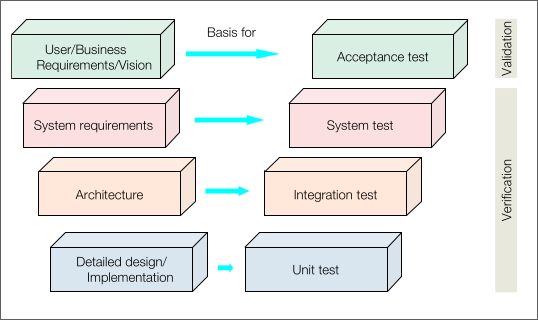
\includegraphics[scale=0.4]{2022-11-14-08:38:52.png}\newline
The base idea is that you need to want to test each "functionality" \textbf{at the lowest level possible!}\newline
Therefore prefer unit tests if possible, but move up through the levels if these aren't enough!
\\
\hline
Validation vs Verification & 
Obviously, just because the tests are good doesn't mean that the product is "validated" by the customer, it might just plain suck.\newline
On the other hand, the customer might not care about that 1 strange test not passing, if the product works well for them.\\
\hline
\end{tabular}
\end{table}
\pagebreak
\begin{table}[ht!]
\begin{tabular}{|m{0.2\linewidth}|m{0.755\linewidth}|}
\hline
Doubles in testing & 
When testing, you often need a placeholder in order to perform your tests.\newline
Here are a bunch of placeholders to consider:\newline
\begin{itemize}
\item \textcolor{purple}{Dummy}\newline
  Object that is passed around but never actually used.\newline
  Usually this is just used to fill parameter lists.
\item \textcolor{purple}{Fake}\newline
  Object that actually have working implementation, but usually take some shortcut,\newline
  which makes them not suitable for production
\item \textcolor{purple}{Stubs}\newline
  Provide answers to calls made during the test.
\item \textcolor{purple}{Mocks}\newline
  Pre-programmed objects with expectations which form a specification of the calls they are expected to receive.
\vspace{-3mm}
\end{itemize} \\
\hline
Black-Box vs White-Box & 
The black box method \textbf{hides the internal structure}, this means that tests can't directly call random functions from the interal structure, instead it has to work with the proper API that any user would.\newline
On the other hand the white box approach is the opposite, where \textbf{the entire internal structure is free game to use.}\newline
Usually \textbf{black box approaches are used with system tests} and \textbf{white box approaches are used for unit tests} and lower level testing.\newline
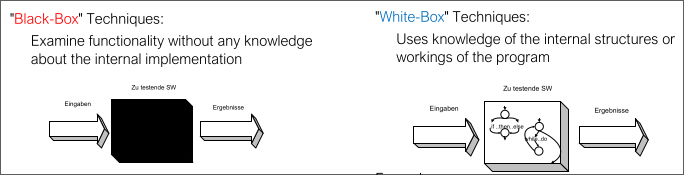
\includegraphics[scale=0.4]{2022-11-14-09:40:32.png}\\
\hline
Black Box techniques & 
\textcolor{OliveGreen}{Equivalence Class Partitioning}\newline
A set of inputs that should show similar behavior.\newline
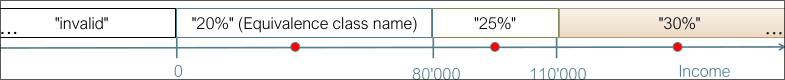
\includegraphics[scale=0.4]{2022-11-14-09:43:48.png}\newline
\textcolor{OliveGreen}{Boundary Value Analysis}\newline
This tests the edges of the classes, making sure that the proper turning point has been chosen.\newline
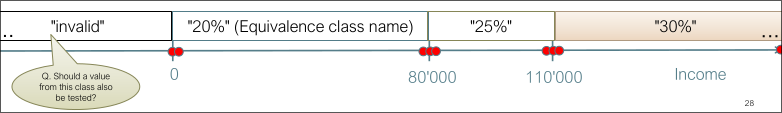
\includegraphics[scale=0.4]{2022-11-14-09:45:41.png}\newline

\\
\hline

\hline

\hline

\hline

\hline

\hline

\hline

\hline

\hline
\end{tabular}
\end{table}
\end{document}

